\pagebreak
\section{Performance comparison of Hadoop vs. Spark on AWS.} \label{T3}
\paragraph{}To perform this comparison, we run the WordCount script 3 times on each file for both Hadoop and Spark to get an approximate average run-time for each file. Again, these tests were made on the AWS Instance, but have also been done locally to confirm their validity. Here is a graph comparing Hadoop and Spark performances.\\
\begin{center}
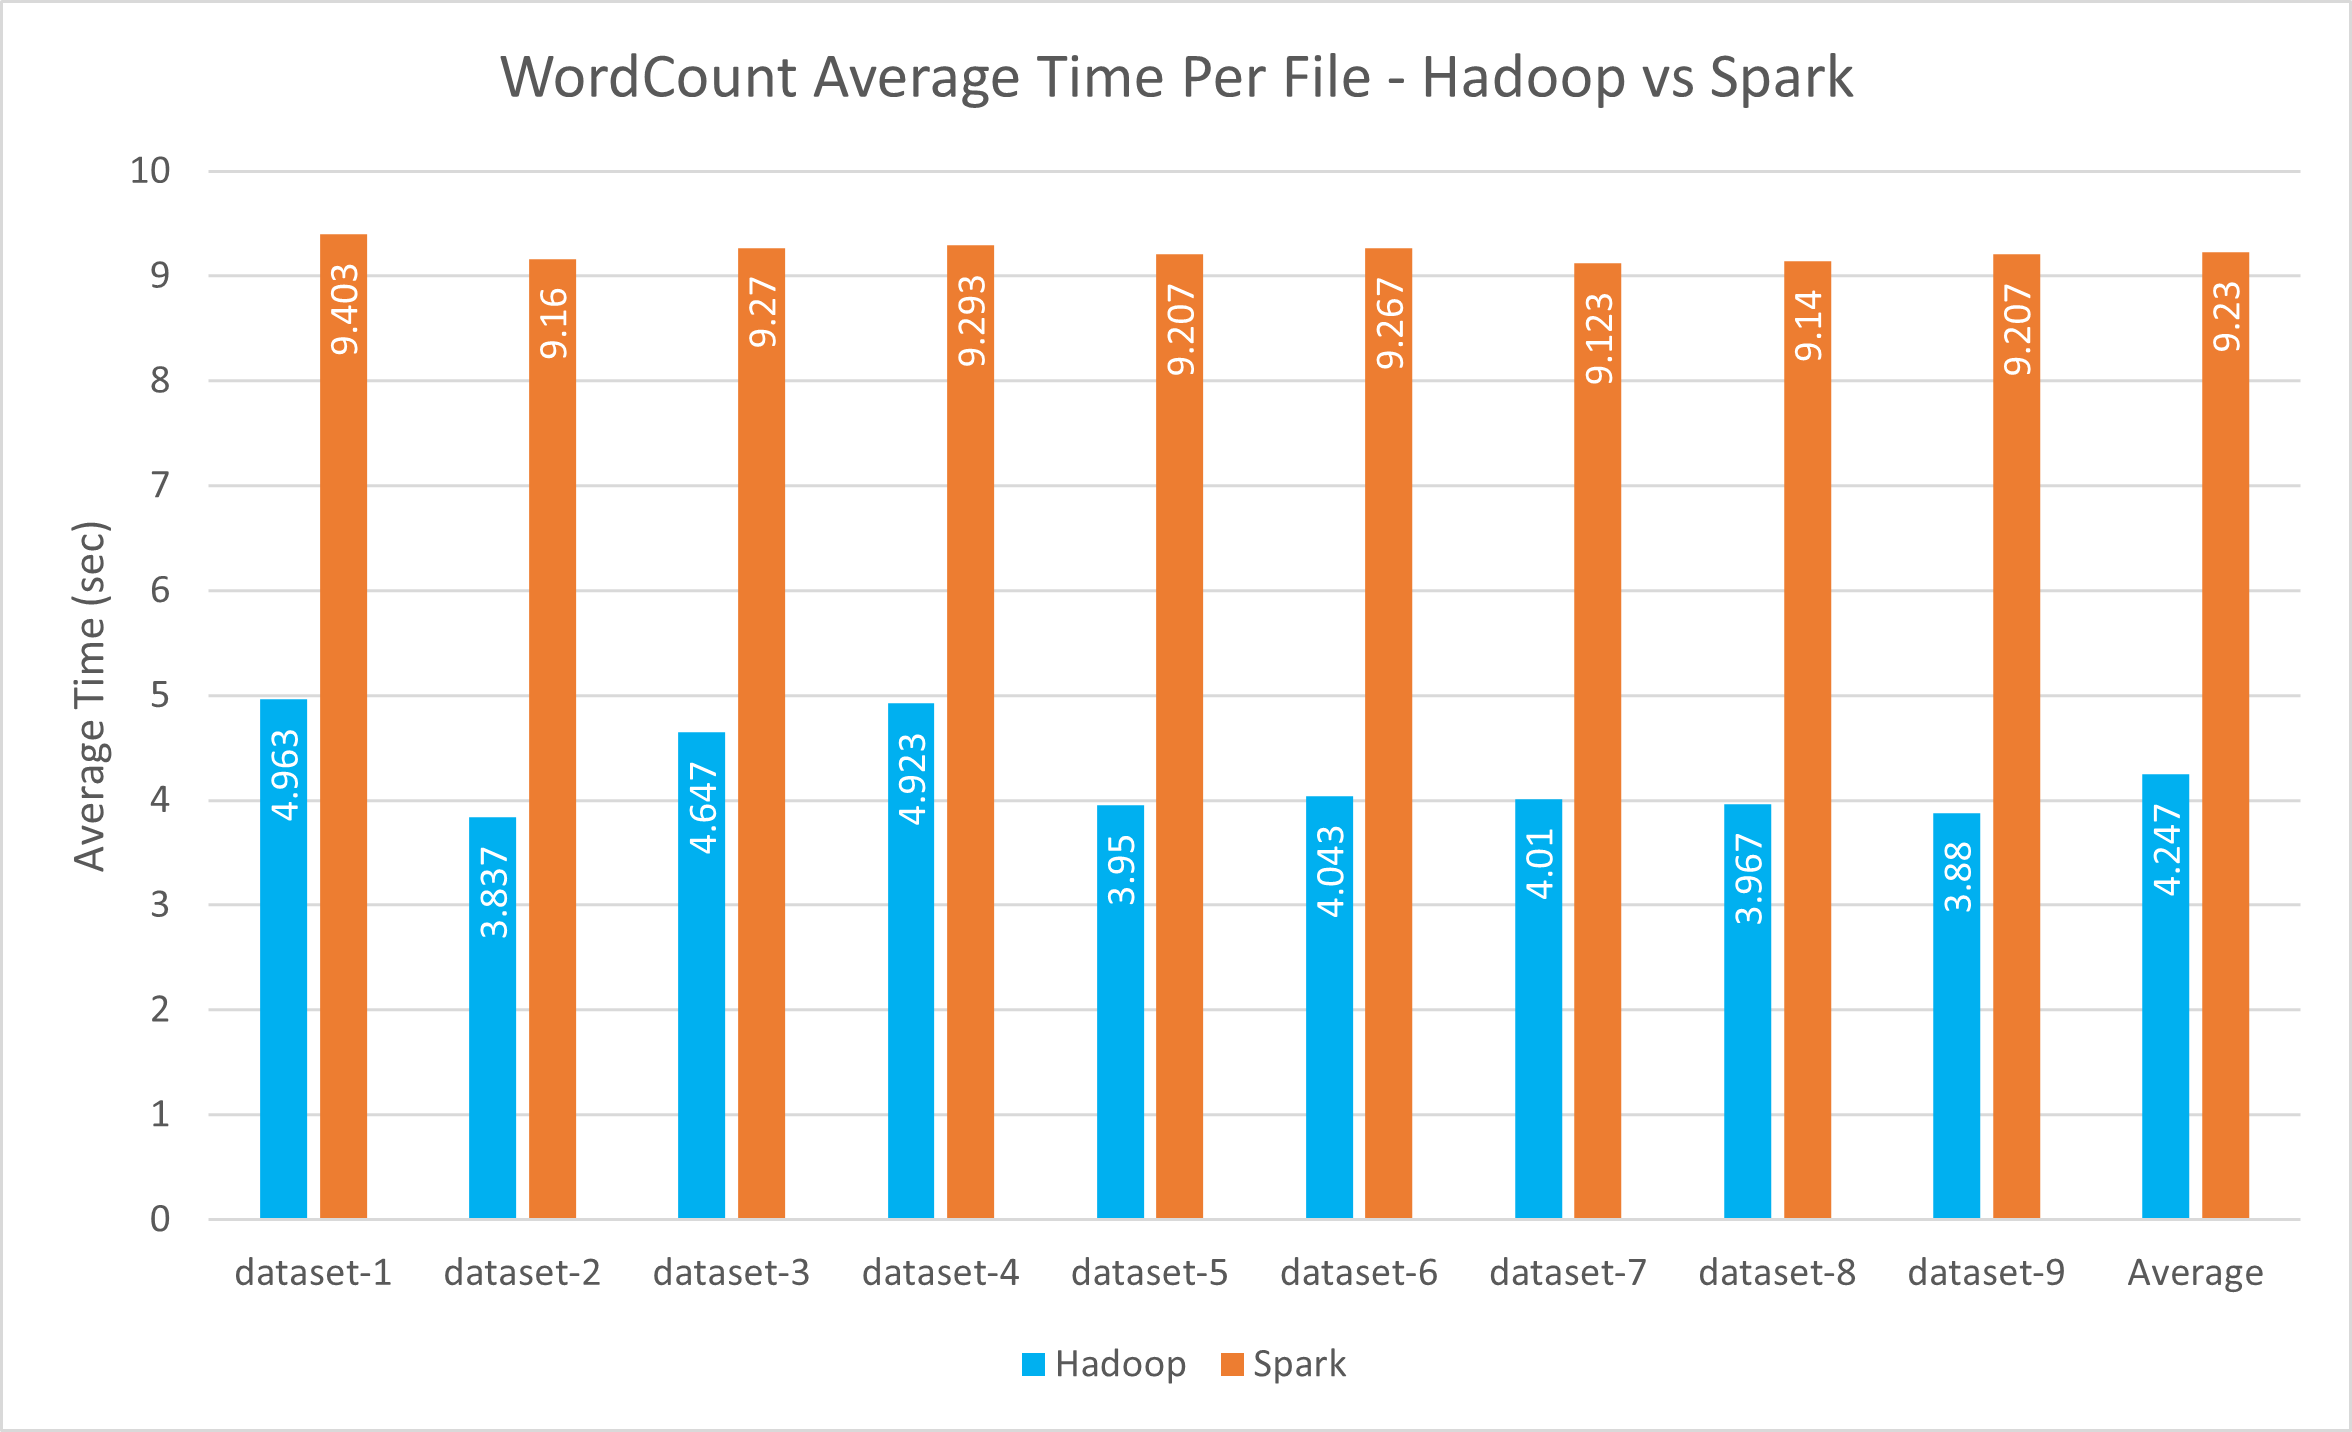
\includegraphics[width=14cm]{Resources/hadoop_vs_spark.png}\\
\emph{Figure 3.1 - Linux vs Hadoop average time}
\end{center}
\paragraph{}From the above graph, we can conclude that Hadoop is about 2 times faster than Spark. This is in contradiction with what we tought would happen, as Spark is known to be able to run up to 100 times faster than Hadoop. This once again can be explained by the fact that Spark has to load the dataset in memory and make connections between everything it has loaded in memory, which are two very expensive operations. With a very large dataset, this step would have a minimal impact over the whole task, but since our dataset is very small, these two steps have a large impact on the results.